
\documentclass{article} % For LaTeX2e
\usepackage{iclr2027_conference,times}

% Optional math commands from https://github.com/goodfeli/dlbook_notation.
\input{math_commands.tex}

\usepackage{hyperref}
\usepackage{url}
\usepackage{algorithm}
\usepackage{algorithmic}
\usepackage{graphicx}
\usepackage{float}

\title{AudioMouth: Language-Assisted Speech-Driven Mouth Animation with Multimodal Language Models}

% Authors must not appear in the submitted version. They should be hidden
% as long as the \iclrfinalcopy macro remains commented out below.
% Non-anonymous submissions will be rejected without review.

\author{Antiquus S.~Hippocampus, Natalia Cerebro \& Amelie P. Amygdale \thanks{ Use footnote for providing further information
about author (webpage, alternative address)---\emph{not} for acknowledging
funding agencies.  Funding acknowledgements go at the end of the paper.} \\
Department of Computer Science\\
Cranberry-Lemon University\\
Pittsburgh, PA 15213, USA \\
\texttt{\{hippo,brain,jen\}@cs.cranberry-lemon.edu} \\
\And
Ji Q. Ren \& Yevgeny LeNet \\
Department of Computational Neuroscience \\
University of the Witwatersrand \\
Joburg, South Africa \\
\texttt{\{robot,net\}@wits.ac.za} \\
\AND
Coauthor \\
Affiliation \\
Address \\
\texttt{email}
}

% The \author macro works with any number of authors. There are two commands
% used to separate the names and addresses of multiple authors: \And and \AND.
%
% Using \And between authors leaves it to \LaTeX{} to determine where to break
% the lines. Using \AND forces a linebreak at that point. So, if \LaTeX{}
% puts 3 of 4 authors names on the first line, and the last on the second
% line, try using \AND instead of \And before the third author name.

\newcommand{\fix}{\marginpar{FIX}}
\newcommand{\new}{\marginpar{NEW}}

%\iclrfinalcopy % Uncomment for camera-ready version, but NOT for submission.
\begin{document}


\maketitle

\begin{abstract}
Speech-driven facial animation aims to recover fine-grained articulation from audio, yet existing methods largely learn this mapping 
from acoustic features while leaving the linguistic structure of speech implicit. Such direct audio-to-motion learning can obscure 
phoneme-specific articulation and weaken local correspondence in long utterances, while token-level objectives do not explicitly 
supervise the dynamics or geometry of complete motion sequences.
We present \textbf{AudioMouth}, a language-assisted framework that formulates audio-to-motion synthesis as schema-constrained sequence 
generation with a multimodal language model.  
To expose the articulatory structure underlying speech, AudioMouth first decomposes 
long recordings into semantically coherent and temporally aligned units comprising audio, transcripts, phonemes, and target motion.
The model is then trained to generate fixed-schema coefficient sequences with explicit phoneme-to-articulation guidance and a 
distribution-balanced objective that mitigates the dominance of frequently occurring low-valued coefficients.
To complement token-level supervision with motion-level feedback, we further refine the generated 
sequences using Group Relative Policy Optimization. The motion-level reward jointly evaluates coefficient reconstruction, 
velocity, acceleration, and a simplified lip-geometry discrepancy that measures 3D mouth deformation in a fixed blendshape 
space without requiring rendering or landmark detection.
On the selected data with a subject-disjoint split, AudioMouth outperforms four Audio2ARKit baselines across all five reported metrics,
reducing Fr\'echet distance from $25.228$ to $10.820$. These results indicate that language-guided structured generation and sequence-level motion
supervision tackle complementary sources of error in speech-driven mouth animation.
\end{abstract}

\section{Introduction}
\label{sec:introduction}
\label{sec:intro}

Speech-driven facial animation aims to generate temporally synchronized facial motion from speech audio, supporting applications in digital avatars and embodied interaction.
Recent advances in portrait animation~\cite{ji2021audio,zhang2023sadtalker}, 3D facial animation~\cite{fan2022faceformer,xing2023codetalker}, and audio-conditioned neural rendering~\cite{guo2021ad} have improved the quality of generated talking faces.
In parallel, compact facial representations, including 3D morphable models, FLAME, and blendshape parameterizations, provide practical control spaces for reconstruction and animation~\cite{blanz2023morphable,li2017learning,menzel2022automated}.
Within blendshape-based representations, ARKit defines semantically meaningful facial action coefficients~\cite{apple_arkit}, offering an interpretable interface between speech articulation and mouth motion.

Existing audio-driven methods predict facial motion from learned acoustic representations, leaving linguistic and articulatory structure implicit in the input waveform~\cite{cudeiro2019voca,richard2021meshtalk,fan2022faceformer,park2023said}.
Viseme-based approaches explicitly model phonetic groups~\cite{zhou2018visemenet}, and more recent methods incorporate textual or linguistic cues~\cite{fan2022joint,xu2024kmtalk}.
However, we observe that relatively little research has explored how aligned audio, transcripts, and phonemes can jointly guide a multimodal language model to generate interpretable ARKit motion trajectories.
This leads us to ask: \emph{Can a multimodal language model use explicit linguistic and articulatory structure to generate accurate mouth-motion trajectories from speech?}

Bearing this in mind, we consider the connection between phonetic units and the facial actions involved in their production.
Bilabial consonants involve lip closure, open vowels generally require greater jaw opening, and transitions between phonemes shape the evolution of mouth motion.
These articulatory relations suggest a natural connection between linguistic inputs and the action semantics of ARKit coefficients.
Recent language-aware facial models provide further motivation: SemanticFace uses language-aligned semantic supervision to estimate facial actions from images~\cite{kang2026semanticface}, while KeyframeFace incorporates language-model priors and semantic keyframes for text-driven facial animation~\cite{wu2025keyframeface}.
Together, these connections motivate us to make transcripts, phonemes, and articulation guidance explicit inputs to a model that generates facial controls. 
Realizing this idea requires both local alignment and suitable training objectives.
Long recordings must be organized into units in which linguistic content and motion targets share temporal boundaries.
Furthermore, low-valued coefficients dominate the training targets and can bias token-level learning.
Even with suitable conditioning, next-token supervision does not explicitly evaluate the temporal dynamics or geometric effects of the resulting trajectories.
These considerations motivate a framework that combines aligned inputs, balanced coefficient generation, and motion-level feedback.

To this end, we present AudioMouth, a language-assisted framework that formulates the prediction of 32 mouth-related ARKit blendshape trajectories as schema-constrained generation with a multimodal language model.
AudioMouth first segments long utterances into semantically coherent units and uses shared temporal boundaries to extract aligned audio, transcript, phoneme, and coefficient subsequences.
The generator then predicts fixed-schema coefficient sequences under explicit phoneme-to-articulation guidance.
A distribution-balanced supervised objective reweights coefficient-value tokens to reduce the dominance of frequently occurring low-valued targets.
To connect token-level learning with the quality of generated motion, we further refine the generator using Group Relative Policy Optimization (GRPO).
The reward compares sampled trajectories with reference motion in terms of coefficient reconstruction, velocity, acceleration, and mouth geometry.
For geometric feedback, we introduce a simplified lip-geometry discrepancy (SLMD) that maps coefficient differences to weighted mouth-vertex displacements through a fixed blendshape basis.
This provides a 3D geometric surrogate without rendering or landmark detection and complements coefficient-wise and temporal supervision. Our contributions are threefold:
\begin{itemize}
    \item We propose AudioMouth, a language-assisted framework that integrates aligned linguistic inputs and explicit articulation guidance into the structured generation of mouth-related ARKit trajectories with a multimodal language model.

    \item We develop a three-stage framework that combines audio-linguistic unit construction, distribution-balanced supervised generation, and motion-aware policy refinement. We introduce SLMD to provide geometric feedback directly from coefficient-induced mouth deformation.

    \item On the selected data, AudioMouth outperforms four Audio2ARKit baselines across all five reported metrics, reducing Fr\'echet distance from the best baseline value of $25.228$ to $10.820$. Ablations support the benefits of linguistic and articulatory conditioning and show additional improvements in distributional and geometric fidelity after motion-aware refinement.
\end{itemize}
  
\section{Related Work}
\noindent\textbf{Speech-Driven 3D Facial Animation.}
Speech-driven 3D facial animation seeks to generate temporally synchronized facial motions from audio. Early approaches formulated the task as direct regression from acoustic features to facial geometry. VOCA~\cite{cudeiro2019voca} predicts speaker-specific 3D vertices, while MeshTalk~\cite{richard2021meshtalk} introduces a categorical latent space for non-verbal motions. Transformer-based models later improved long-range temporal modeling: FaceFormer~\cite{fan2022faceformer} employs an autoregressive transformer, and UniTalker~\cite{fan2024unitalker} enables unified training across datasets.
A key challenge is the inherent one-to-many mapping from audio to facial motion, which often leads to over-smoothed results. To address this, CodeTalker~\cite{xing2023codetalker} incorporates discrete motion priors via vector quantization. Diffusion-based methods such as SAiD~\cite{park2023said} and FaceDiffuser~\cite{stan2023facediffuser} better capture motion diversity and stochasticity. In production settings, NVIDIA Audio2Face-3D~\cite{chung2025audio2face} provides a robust real-time pipeline, while SentiAvatar~\cite{jin2026sentiavatar} introduces planning strategies for improved semantic consistency at the sentence level. More recently, Ex-Omni~\cite{zhang2026ex}, where the omni-modal mainly provides semantic understanding and speech-unit representations, employs a separate lightweight facial generator that maps these units to blendshape coefficients.
Building on these advances, AudioMouth formulates mouth-motion prediction as fixed-schema coefficient generation with a multimodal language model conditioned on audio and explicit linguistic inputs. We complement token-level supervision with sequence-level refinement that evaluates the generated trajectories in coefficient, temporal, and geometric terms.

\noindent\textbf{Facial Motion Representations.}
The choice of facial motion representation significantly impacts controllability, interpretability, and compatibility with modern multimodal models. Vertex-based representations~\cite{cudeiro2019voca,fan2022faceformer} preserve fine geometric details but lack semantic interpretability. Parametric models such as FLAME~\cite{li2017learning} achieve compactness via PCA, yet their latent dimensions are not naturally aligned with linguistic or phonetic concepts.
ARKit blendshapes~\cite{apple_arkit} provide semantically meaningful facial action controls, such as jaw opening, cheek puffing, and mouth closure, while SemanticFace~\cite{kang2026semanticface} demonstrates the benefit of language-aligned supervision for estimating these coefficients from images.
AudioMouth adopts 32 mouth-related ARKit channels as an interpretable output space that connects articulatory cues with explicit facial controls. This coefficient space also supports SLMD, which measures the resulting mouth deformation through a fixed blendshape basis.

\noindent\textbf{Linguistic and Articulatory Priors.}
Speech articulation is fundamentally tied to phonetic and linguistic structure: bilabial consonants involve lip closure, open vowels generally require greater jaw opening, and phoneme transitions shape temporal dynamics~\cite{cohen1993modeling,taylor2012dynamic,edwards2016jali}. Classic and viseme-based approaches~\cite{cohen1993modeling,edwards2016jali,taylor2017deep,zhou2018visemenet,bao2023learning} explicitly leverage these relations to guide speech animation.
Recent works incorporate higher-level cues. Emotion- and sentiment-aware methods~\cite{peng2023emotalk,jin2026sentiavatar} add control signals beyond raw audio, demonstrating the value of non-acoustic information. Recent audio-text or linguistically guided methods~\cite{fan2022joint,xu2024kmtalk} further suggest that textual or linguistic cues can reduce the ambiguity of audio-to-motion generation.
AudioMouth brings these cues into temporally aligned training units containing audio, transcripts, phonemes, and target coefficients. Within each unit, explicit phoneme-to-articulation guidance conditions coefficient generation alongside the acoustic input, while a distribution-balanced objective addresses the imbalance in coefficient values.

\section{Method}
\label{sec:method}

To connect speech articulation with explicit linguistic structure, AudioMouth generates mouth-related ARKit trajectories through the three-stage pipeline in Figure~\ref{fig:overview}.
The left column summarizes the pipeline. The three modules on the right address local audio-linguistic alignment, articulatory conditioning and coefficient imbalance, and sequence-level motion supervision, respectively.
We first formulate the prediction task, then describe these modules in order; Algorithm~\ref{alg:framework} summarizes training and inference.

\begin{figure*}[h]
    \centering
    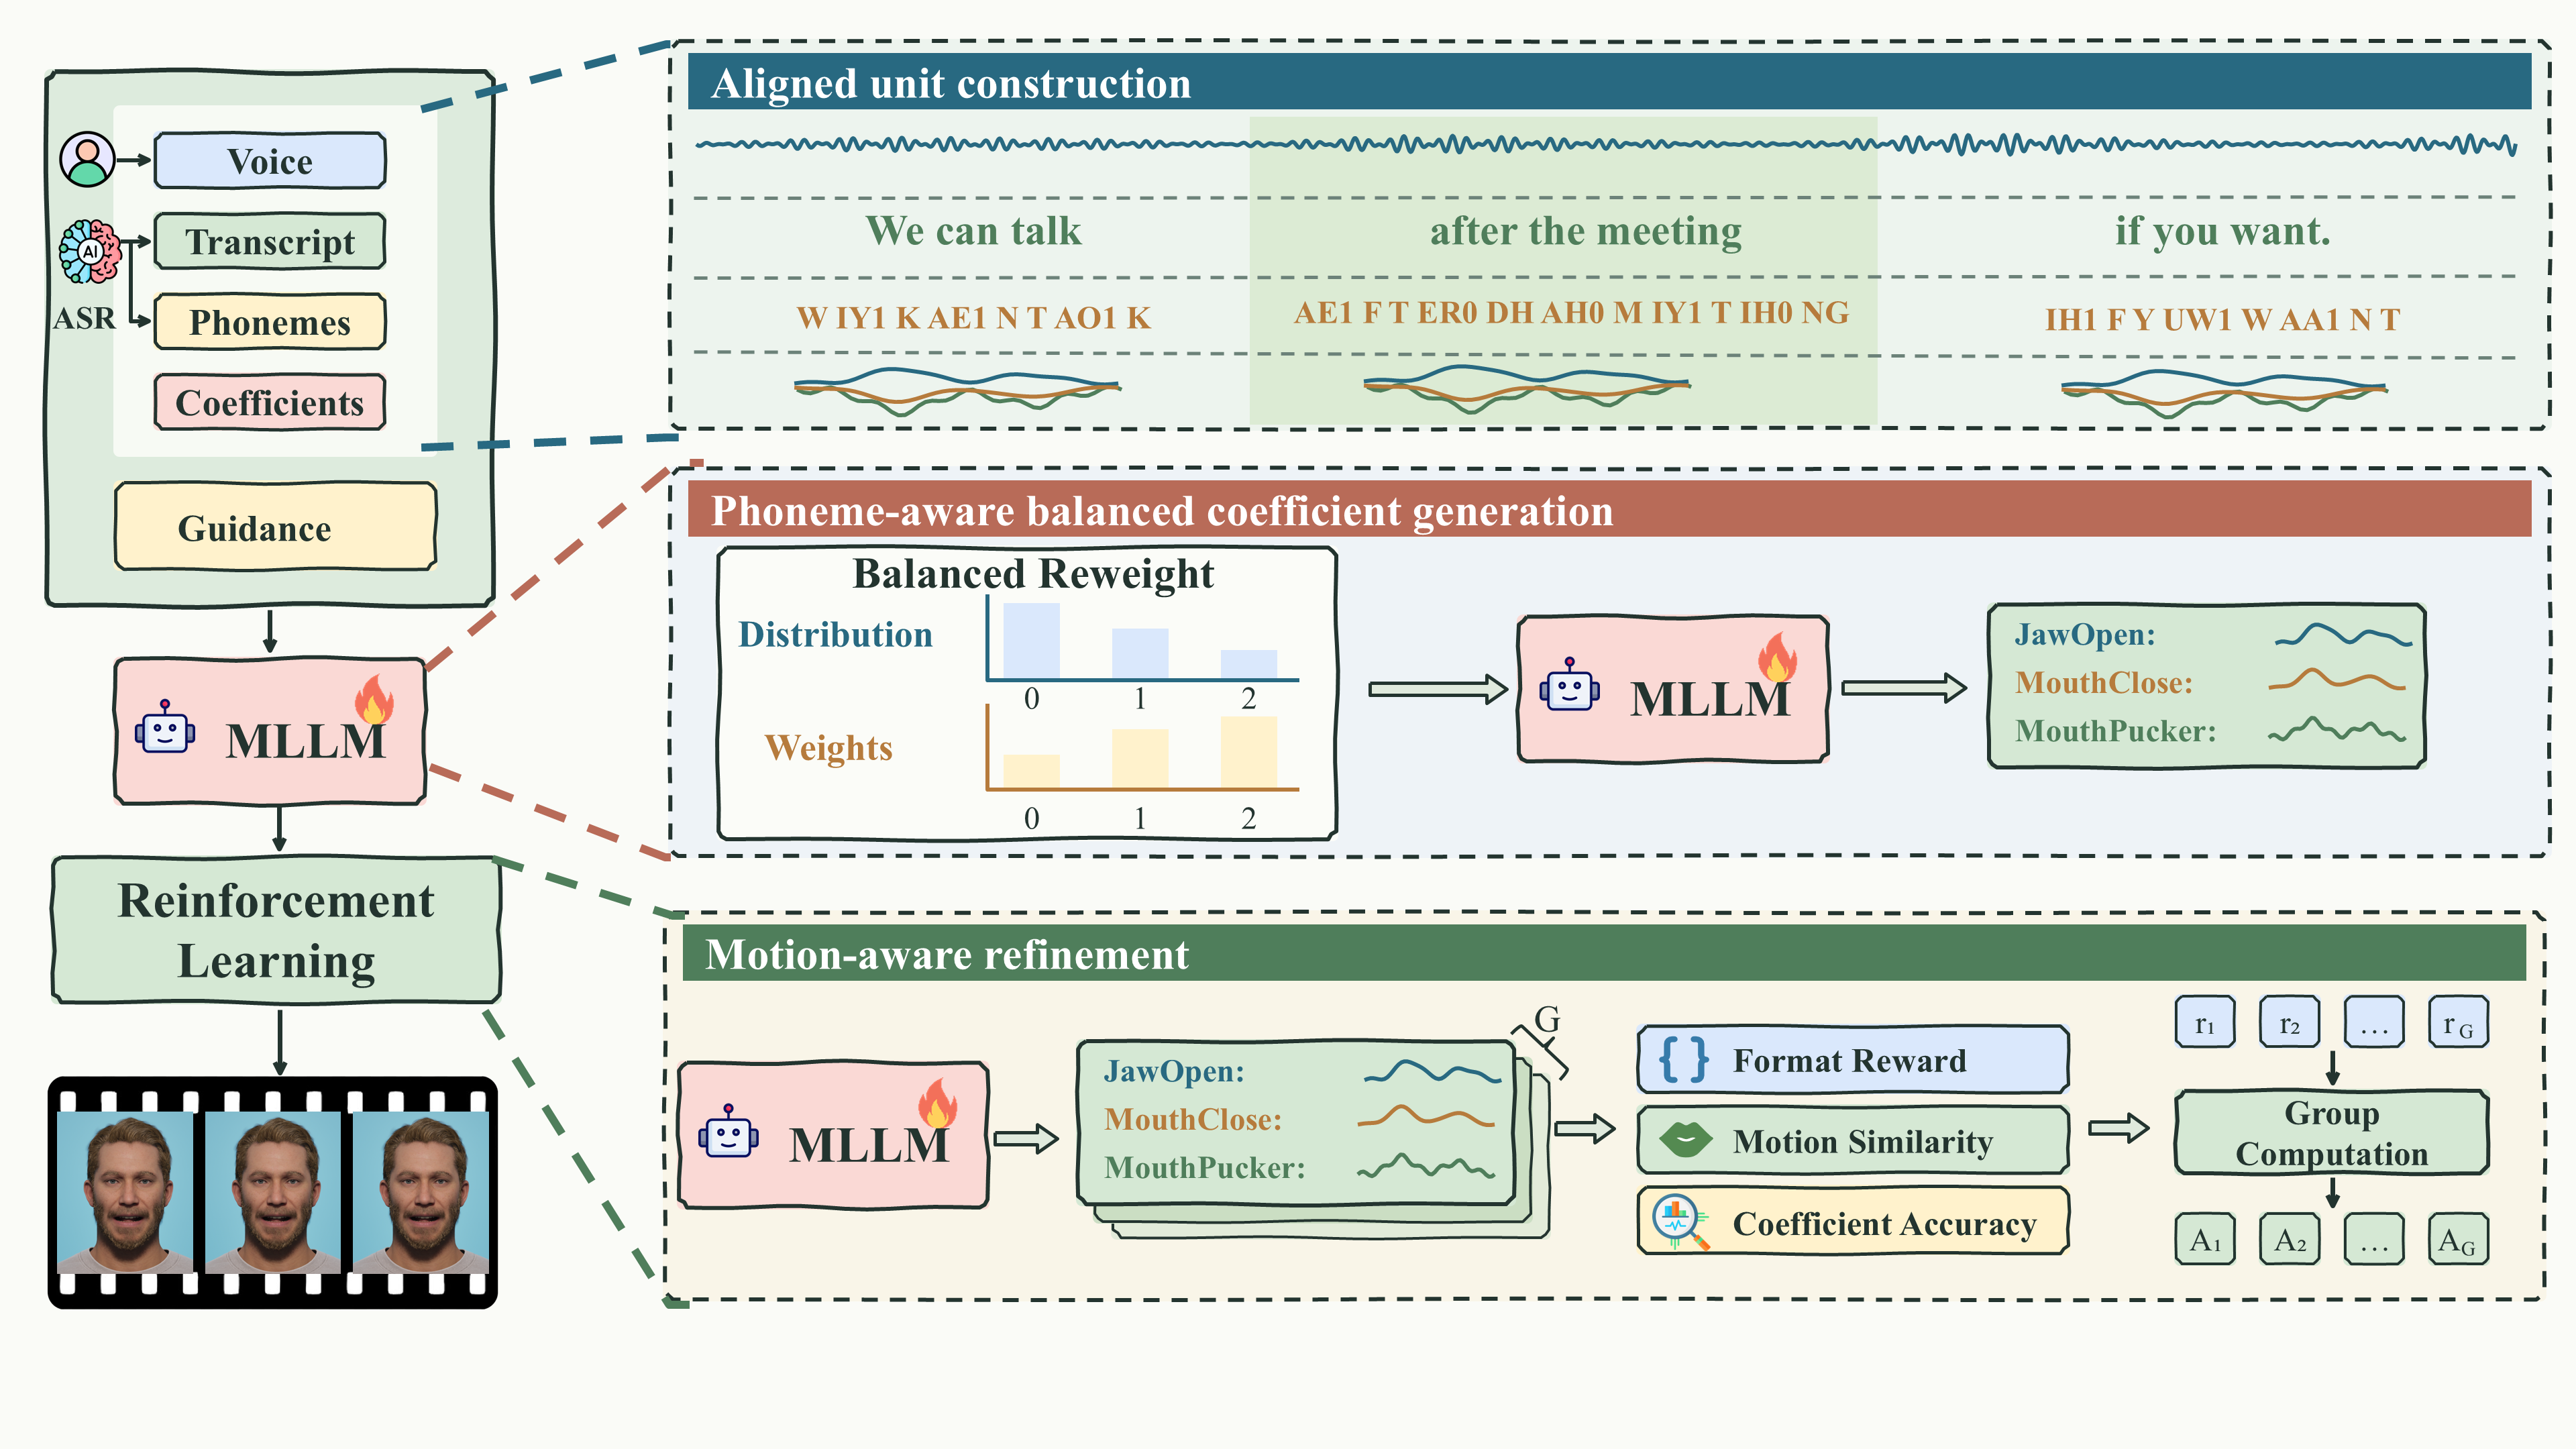
\includegraphics[width=\textwidth]{img/method.png}
    \caption{
Overview of AudioMouth. The left column shows the overall pipeline. The upper-right module constructs aligned audio-linguistic units, the middle-right module learns phoneme-aware coefficient generation with distribution-balanced supervision, and the lower-right module refines sampled sequences through group-relative policy updates using format validity and motion-quality feedback. At inference, the refined generator predicts segment-level coefficients, which are concatenated and post-processed for animation.
    }
    \label{fig:overview}
\end{figure*}

\subsection{Problem Formulation}
\label{sec:problem_formulation}

Given a speech waveform $\mathcal{A}=\{a_n\}_{n=1}^{N}$ and aligned linguistic inputs, our goal is to predict a synchronized coefficient sequence $\mathcal{V}=\{v_t\}_{t=1}^{T}$, where $v_t\in\mathbb{R}^{K}$ contains $K=32$ mouth-related ARKit controls.
Here, $N$ and $T$ denote the numbers of audio samples and motion frames, respectively; paired coefficient sequences provide supervision during training.
We divide each recording into $J$ aligned units, with segment-level inputs and targets
\[
\mathcal{X}^j=(\mathcal{A}^j,w^j,\mathcal{P}^j), \qquad
\mathcal{Y}^j=\mathrm{Serialize}_{\mathrm{json}}(\mathcal{V}^j),
\]
where $w^j$ and $\mathcal{P}^j$ are the transcript and phoneme sequence associated with audio segment $\mathcal{A}^j$, and $\mathcal{V}^j$ is its target motion.
To express motion as a structured sequence for the MLLM, we serialize each ARKit channel as a predefined JSON key with a temporally ordered sequence of coefficient values.
The MLLM models the resulting token sequence $\mathcal{Y}^j=(y_1,\ldots,y_{M_j})$ autoregressively:
\begin{equation}
p_\theta(\mathcal{Y}^j\mid\mathcal{X}^j)
=\prod_{m=1}^{M_j}p_\theta(y_m\mid y_{<m},\mathcal{X}^j),
\label{eq:structured_generation}
\end{equation}
where $\theta$ denotes the generator parameters, $M_j$ is the output token length, and $y_{<m}$ denotes the preceding tokens.
The conditioning also includes the articulation guidance described in Section~\ref{sec:stage2}, omitted from the notation for brevity.

This formulation requires local correspondence between the conditioning signals and target motion.
Moreover, frequent low-valued coefficients can dominate token-level supervision, while token likelihood alone does not measure the geometry or dynamics of a generated sequence.
The following three modules address alignment, coefficient imbalance, and motion-level supervision, respectively.

\subsection{High-Quality Audio-Linguistic Unit Construction}
\label{sec:stage1}

To preserve local correspondence between linguistic content and motion across long recordings, we construct aligned audio-linguistic units in the upper-right module of Figure~\ref{fig:overview}.
Semantic boundaries retain coherent utterances, while shared timestamps associate their speech sounds with the corresponding motion targets.

\paragraph{Semantic Segmentation and Temporal Alignment.}
For general and in-the-wild recordings, ASR provides the transcript $\tilde{W}$ and word-level timestamps $\tau$, and SAT partitions the transcript into semantically coherent segments $\mathcal{W}=\{w^j\}_{j=1}^{J}$.
The shared temporal boundaries align each audio segment $\mathcal{A}^j$ with its transcript $w^j$, associated phoneme sequence $\mathcal{P}^j$, and training motion target $\mathcal{V}^j$.
These units provide local linguistic and motion correspondence for coefficient generation. At inference, the same input construction omits the target motion.

\subsection{Phoneme-Aware Balanced Coefficient Generation}
\label{sec:stage2}

To translate the aligned linguistic cues into facial controls while reducing bias toward frequent coefficient values, we combine phoneme-aware conditioning with distribution-balanced supervision.
The middle-right module of Figure~\ref{fig:overview} implements these two components through supervised fine-tuning (SFT) of the conditional distribution in Eq.~\ref{eq:structured_generation}.

\paragraph{Phoneme-Aware Conditioning.}
To make the relationship between speech sounds and facial actions explicit, we condition the MLLM on the audio segment $\mathcal{A}^j$, transcript $w^j$, phonemes $\mathcal{P}^j$, and phoneme-to-articulation guidance.
The guidance links phonetic categories to actions such as lip closure for bilabial phonemes and larger jaw opening for open vowels, while audio supplies the acoustic evidence for the generated trajectories.

\paragraph{Distribution-Balanced Supervision.}
To prevent frequent low-valued coefficients from dominating next-token supervision, we reduce their loss contribution using a fixed coefficient-value weighting function $\omega$.
The distribution and weight plots in Figure~\ref{fig:overview} illustrate this imbalance and the corresponding reweighting.
Weights apply only to tokens representing trajectory values; schema-related tokens retain unit weight.
The training objective is
\begin{equation}
\mathcal{L}_{\mathrm{DB}} = -\sum_{m=1}^{M_j}\omega(y_m)\log p_\theta(y_m\mid y_{<m},\mathcal{X}^j).
\label{eq:db_sft}
\end{equation}
This objective balances coefficient-value supervision while preserving the output schema and conditioning inputs.
The resulting parameters $\theta_{\mathrm{SFT}}$ initialize the subsequent refinement stage.

\begin{algorithm}[t]
\caption{AudioMouth Training and Inference}
\label{alg:framework}
\small
\begin{algorithmic}[1]
\REQUIRE Paired data $\mathcal{D}$, pretrained MLLM $\theta_0$, test speech $\mathcal{A}_{\mathrm{test}}$
\ENSURE Refined generator $\theta_{\mathrm{GRPO}}$ and predicted coefficients $\hat{\mathcal{V}}$
\STATE \textbf{Aligned Unit Construction:} $\mathcal{U}\leftarrow\emptyset$
\FOR{each $(\mathcal{A},\mathcal{V})\in\mathcal{D}$}
    \STATE $(\tilde{W},\tau)\leftarrow\mathrm{ASR}(\mathcal{A})$; $\mathcal{W}\leftarrow\mathrm{SAT}(\tilde{W})$
    \STATE Add aligned units $(\mathcal{X}^j,\mathcal{V}^j,\mathcal{Y}^j)$ to $\mathcal{U}$ using Section~\ref{sec:stage1}
\ENDFOR
\STATE \textbf{Phoneme-Aware Balanced Coefficient Generation}
\STATE Set fixed coefficient-value weights $\omega$ for distribution-balanced supervision
\STATE $\theta_{\mathrm{SFT}}\leftarrow\mathrm{SFT}(\theta_0,\mathcal{U},\omega)$ using Eq.~\ref{eq:db_sft} and articulation guidance
\STATE \textbf{Motion-Aware Refinement:} $\theta\leftarrow\theta_{\mathrm{SFT}}$
\FOR{each training unit $(\mathcal{X}^j,\mathcal{V}^j,\mathcal{Y}^j)\in\mathcal{U}$}
    \STATE Sample $G$ candidates $\{\hat{\mathcal{Y}}^j_i\}_{i=1}^{G}\sim p_\theta(\cdot\mid\mathcal{X}^j)$
    \STATE Parse candidates and compute $\{r_i\}_{i=1}^{G}$ against $\mathcal{V}^j$, with validity and length handling
    \STATE $\hat{A}_i\leftarrow(r_i-\bar{r})/(\sigma_r+\epsilon)$ for each candidate
    \STATE Update $\theta$ with GRPO using $\{\hat{A}_i\}_{i=1}^{G}$ (Section~\ref{sec:stage3})
\ENDFOR
\STATE $\theta_{\mathrm{GRPO}}\leftarrow\theta$
\STATE \textbf{Inference}
\STATE Construct $\{\mathcal{X}^j\}_{j=1}^{J}$ from $\mathcal{A}_{\mathrm{test}}$ using Section~\ref{sec:stage1}
\STATE Generate $\hat{\mathcal{Y}}^j$ with $\theta_{\mathrm{GRPO}}$ and parse into $\hat{\mathcal{V}}^j$ for each unit
\STATE $\hat{\mathcal{V}}\leftarrow\mathrm{PostProcess}(\mathrm{Concat}(\{\hat{\mathcal{V}}^j\}_{j=1}^{J}))$ in temporal order
\end{algorithmic}
\end{algorithm}

\subsection{Motion-Aware Refinement}
\label{sec:stage3}

To supervise the temporal dynamics and mouth geometry that token likelihood does not directly measure, we refine the SFT generator with sequence-level motion rewards using Group Relative Policy Optimization (GRPO), as shown in the lower-right module of Figure~\ref{fig:overview}.
Starting from $\theta_{\mathrm{SFT}}$, we sample $G$ candidate JSON outputs for each input $\mathcal{X}^j$ and compare their decoded trajectories with the reference $\mathcal{V}^j$.
The reward combines coefficient accuracy, temporal dynamics, and mouth geometry for valid candidates; relative rewards within each group guide the policy update.

\paragraph{Simplified Lip-Geometry Discrepancy (SLMD).}
To capture how coefficient errors jointly affect mouth shape, we introduce SLMD, which measures their combined geometric effect through a fixed ARKit blendshape basis.
This provides geometric feedback without rendering candidate videos or detecting landmarks.
Let $\mathbf{C}^{p},\mathbf{C}^{g}\in\mathbb{R}^{T\times K}$ denote candidate and reference sequences expressed in the coefficient convention of this basis.
For each mouth-region vertex $m\in\mathcal{M}$, $\mathbf{b}_{k,m}\in\mathbb{R}^{3}$ is the displacement of the $k$-th blendshape mesh from the neutral mesh.
The shared neutral geometry cancels when comparing the two sequences, giving
\begin{align}
\delta\mathbf{x}_{t,m} &= \sum_{k=1}^{K}(c^p_{t,k}-c^g_{t,k})\mathbf{b}_{k,m}, \label{eq:slmd_displacement}\\
\mathcal{L}_{\mathrm{slmd}} &= \frac{\sum_{t=1}^{T}\sum_{m\in\mathcal{M}}w_m\|\delta\mathbf{x}_{t,m}\|_2}{T\sum_{m\in\mathcal{M}}w_m}. \label{eq:slmd}
\end{align}
Here, $T$ denotes the compared segment length, and the fixed vertex weights $w_m$ emphasize the lips while retaining lower-weight surrounding vertices.
SLMD is thus a weighted mean Euclidean discrepancy in 3D mouth deformation; the basis and weights are reused across candidates.
It supplies a geometric training signal distinct from the rendered-video 2D landmark distance used for evaluation.

\paragraph{Motion-Level Reward.}
To assess both mouth shape and its evolution over time, we combine SLMD with coefficient MSE and first- and second-order temporal difference discrepancies, denoted by $\mathcal{L}_{\mathrm{mse}}$, $\mathcal{L}_{\mathrm{vel}}$, and $\mathcal{L}_{\mathrm{acc}}$.
The temporal terms compare motion changes with the reference rather than penalizing movement itself.
To account for their different numerical scales, each discrepancy is converted into a bounded score before aggregation:
\begin{align}
S_q &= \left(1+\mathcal{L}_q/s_q\right)^{-1}, \label{eq:normalized_score}\\
r_{\mathrm{motion}} &= \sum_{q\in\{\mathrm{mse},\mathrm{vel},\mathrm{acc},\mathrm{slmd}\}}\lambda_q S_q. \label{eq:motion_reward}
\end{align}
The scales $s_q$ are fixed reference medians, and the nonnegative weights $\lambda_q$ sum to one.
Valid candidates receive the motion reward with a length-mismatch penalty when applicable; invalid outputs receive fixed negative penalties.
These operations correspond to the coefficient-accuracy, motion-similarity, and format-reward blocks in Figure~\ref{fig:overview}.

\paragraph{Group-Relative Policy Update.}
To favor higher-quality motion among candidates generated for the same input, we convert their rewards $\{r_i\}_{i=1}^{G}$ into group-relative advantages $\hat{A}_i=(r_i-\bar{r})/(\sigma_r+\epsilon)$, where $\bar{r}$ and $\sigma_r$ are the group mean and standard deviation, and $\epsilon$ ensures numerical stability.
The group-computation block in Figure~\ref{fig:overview} supplies these advantages to the GRPO policy update.
The resulting generator $\theta_{\mathrm{GRPO}}$ retains the structured output representation learned during SFT and is further optimized using motion-level feedback.

\paragraph{Inference.}
Given test speech, we construct the aligned input units and use $\theta_{\mathrm{GRPO}}$ to generate a JSON coefficient sequence for each segment.
To reconstruct a complete trajectory and reduce discontinuities between segments, we concatenate the decoded predictions in temporal order and apply post-processing, completing the pipeline in the left column of Figure~\ref{fig:overview}.
%标题需要把创新的位置推出来
%总页数9页，需要进一步压缩
%标注图采用纵向排版，才用左边一列讲述流程，然后右边一列拉开来细讲
%公式可以全部摆在一行内

\section{Experiments}
\label{sec:experiments}

\begin{figure*}[h]
    \centering
    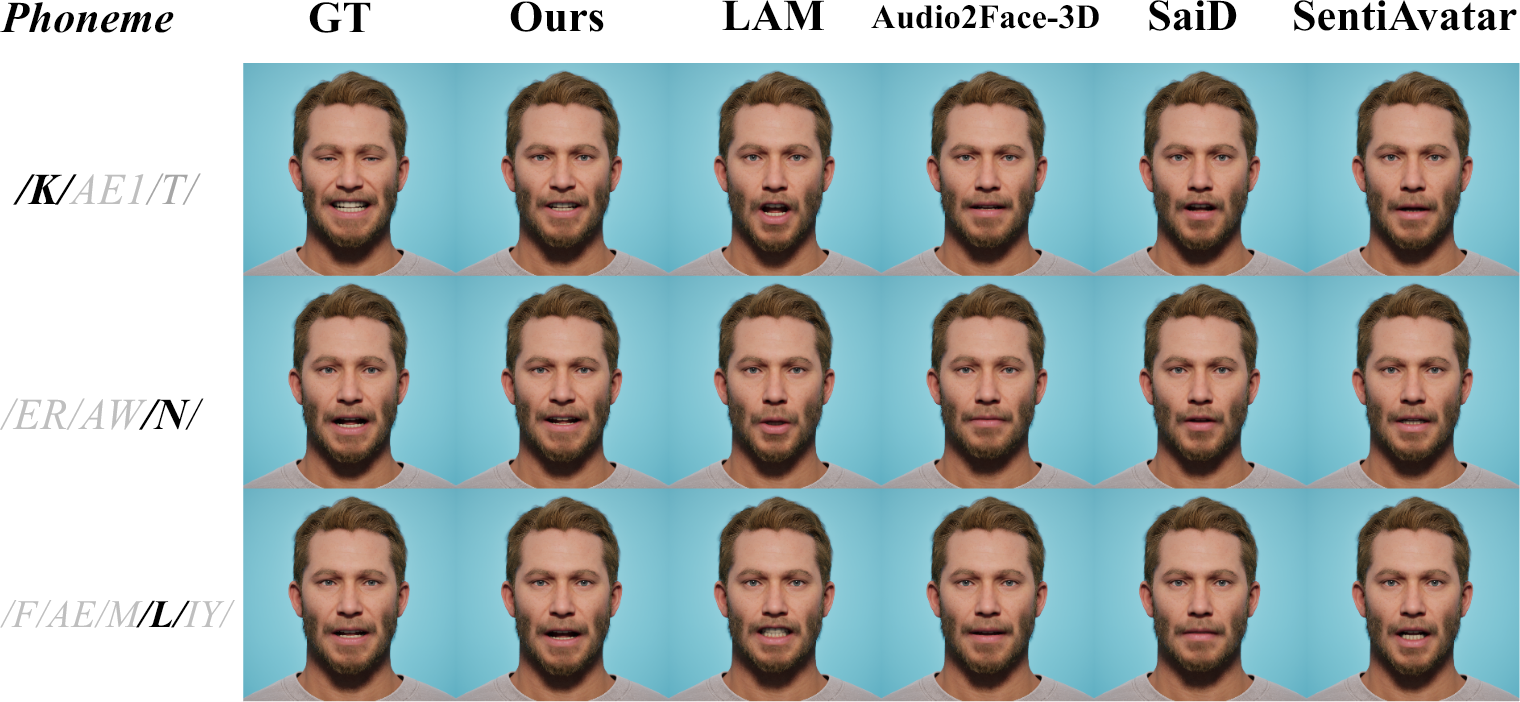
\includegraphics[width=1\linewidth]{comparison.png}
    \caption{
    Qualitative comparison of audio-driven facial animation results.
    From top to bottom, the rows show examples from the words ``cat'', ``around'', and ``family'', respectively.
    The leftmost column shows phoneme annotations, with the active phoneme highlighted in bold black and the surrounding phonemes shown in gray.
    }
    \label{fig:comparison}
\end{figure*}

In this section, we evaluate the proposed language-assisted Audio2ARKit framework through quantitative and qualitative experiments.
We first introduce the dataset used for training and evaluation.
We then describe the experimental setup, including baselines, evaluation metrics, and implementation details.
Next, we compare our method with existing approaches.
Finally, to analyze the contribution of each design component, we conduct ablation studies.


\subsection{Dataset}
\label{subsect:dataset}

We use selected data from BEAT~\cite{liu2022beat} for training and evaluation.

\paragraph{Data Split.}
We use a subject-disjoint split of 277 sequences into 176 training, 40 validation, and 61 test sequences, keeping test speakers unseen during training.
Semantic segmentation yields 21,513 segments: 15,655 for training, 2,858 for validation, and 3,000 for testing.

\subsection{Experimental Setup}
\label{subsect:experimental_setup}

\paragraph{Baselines.}
We compare with SAiD~\cite{park2023said}, Audio2Face-3D~\cite{chung2025audio2face}, LAM-A2E~\cite{lam}, and SentiAvatar~\cite{jin2026sentiavatar}.
Audio2Face-3D, LAM-A2E, and SentiAvatar use their publicly released pretrained weights; SAiD is fine-tuned from its public checkpoint on our training split.

\paragraph{Evaluation Metrics.}
We employ five quantitative metrics to comprehensively evaluate the performance: Mean Squared Error (MSE), Mean Absolute Error (MAE), Fréchet Distance (FD), Wasserstein Inception Distance (WInD), and Lip Landmark Distance (LMD). MSE and MAE measure the frame-level accuracy of the predicted ARKit blendshape coefficients against the ground truth. FD evaluates the distributional discrepancy between the predicted motion sequences and the ground-truth sequences in the extracted feature space. WInD, following the protocol introduced in prior work \cite{park2023said}, provides a robust benchmark for comparing the perceptual quality and temporal dynamics of the generated sequences against the ground truth. LMD measures the mean Euclidean distance between detected 2D mouth landmarks in paired rendered videos.

\paragraph{Implementation Details.}
The general preprocessing pipeline combines ASR with SAT~\cite{frohmann2024segment} for transcript extraction and semantic segmentation.
Our generator is initialized from Qwen3-Omni-30B-A3B-Instruct~\cite{xu2025qwen3omni} and adapted with LoRA~\cite{hu2021lora} on the language decoder, with the audio encoder and multimodal alignment modules frozen.
We train SFT and GRPO for four epochs each on four NVIDIA A100 GPUs, with global batch sizes of 8 and 24, respectively.
GRPO combines coefficient, temporal, and mouth-geometry feedback.


% TODO: Document the exact post-processing switches for the reported result groups.
\subsection{Comparison with Audio2ARKit Methods}
\label{sec:main_comparison}

We compare AudioMouth with four competitive baselines: LAM-A2E~\cite{lam}, NVIDIA Audio2Face-3D~\cite{chung2025audio2face}, SAiD~\cite{park2023said}, and SentiAvatar~\cite{jin2026sentiavatar}. To ensure fair comparison, we extract speaking segments from both ground-truth and generated sequences based on the script and concatenate them, since our method focuses specifically on speech-related mouth motion prediction.

Predictions are concatenated and post-processed as described in Section~\ref{sec:stage3}. In the tables, SFT denotes the generator in the second stage and Refined (GRPO) denotes the generator after refinement; both use the reported post-processing setting.

\begin{table}[t]
\centering
{\fontsize{9}{10.5}\selectfont
\renewcommand{\arraystretch}{1.02}
\begin{tabular*}{\textwidth}{
    @{\extracolsep{\fill}} lccccc @{}
}
\hline
\textbf{Methods}
& \textbf{MSE $\downarrow$}
& \textbf{MAE $\downarrow$}
& \textbf{FD $\downarrow$}
& \textbf{WInD $\downarrow$}
& \textbf{LMD $\downarrow$} \\
\hline

LAM-A2E
& $0.023$
& $0.109$
& $38.403 \pm 10.149$
& $41.751 \pm 10.885$
& $7.648 \pm 0.497$ \\

Audio2Face-3D
& $0.020$
& $0.106$
& $25.228 \pm 3.560$
& $29.879 \pm 4.454$
& $7.879 \pm 0.438$ \\

SAiD
& $0.021$
& $0.108$
& $58.357 \pm 21.580$
& $62.256 \pm 21.911$
& $7.651 \pm 0.504$ \\

SentiAvatar
& $0.022$
& $0.106$
& $40.609 \pm 10.277$
& $42.153 \pm 10.542$
& $8.131 \pm 1.005$ \\

AudioMouth
& $\mathbf{0.006}$
& $\mathbf{0.053}$
& $\mathbf{10.820 \pm 2.635}$
& $\mathbf{16.513 \pm 3.584}$
& $\mathbf{6.249 \pm 0.723}$ \\
\hline
\end{tabular*}
}
\caption{Comparison with Audio2ARKit methods on 60 scripts from the selected test data. AudioMouth is the generator after Sequence-Level Motion Refinement with post-processing. FD, WInD, and LMD are mean $\pm$ sample standard deviation across scripts. Bold indicates the lowest reported value in each column.}
\label{tab:quantitative_results}
\end{table}

% Original table retained for reference; the figure is used in the compiled manuscript.
% \begin{table}[t]
% \centering
% {\fontsize{9}{10.5}\selectfont
% \renewcommand{\arraystretch}{1.02}
% \begin{tabular*}{\textwidth}{@{\extracolsep{\fill}} lccccc @{}}
% \multicolumn{6}{c}{\textbf{(a) Linguistic and Articulatory Conditioning}} \\[0.15em]
% \hline
% \textbf{Methods}
% & \textbf{MSE $\downarrow$}
% & \textbf{MAE $\downarrow$}
% & \textbf{FD $\downarrow$}
% & \textbf{WInD $\downarrow$}
% & \textbf{LMD $\downarrow$} \\
% \hline
%
% w/o Guidance
% & $0.007484$
% & $0.057885$
% & $53.743 \pm 74.384$
% & $62.356 \pm 76.296$
% & $6.917 \pm 0.818$ \\
%
% Audio Only
% & $0.007288$
% & $0.059896$
% & $83.640 \pm 94.524$
% & $93.230 \pm 96.674$
% & $6.938 \pm 0.989$ \\
%
% SFT
% & $\mathbf{0.005978}$
% & $\mathbf{0.053467}$
% & $\mathbf{11.282 \pm 3.888}$
% & $\mathbf{17.052 \pm 4.990}$
% & $\mathbf{6.297 \pm 0.825}$ \\
% \hline
% \end{tabular*}
%
% \vspace{0.5em}
%
% \begin{tabular*}{\textwidth}{@{\extracolsep{\fill}} lccccc @{}}
% \multicolumn{6}{c}{\textbf{(b) Distribution-Balanced Supervision}} \\[0.15em]
% \hline
% \textbf{Methods}
% & \textbf{MSE $\downarrow$}
% & \textbf{MAE $\downarrow$}
% & \textbf{FD $\downarrow$}
% & \textbf{WInD $\downarrow$}
% & \textbf{LMD $\downarrow$} \\
% \hline
%
% w/o Reweighting
% & $0.012226$
% & $0.074727$
% & $21.663 \pm 8.109$
% & $29.253 \pm 7.603$
% & $9.011 \pm 0.630$ \\
%
% SFT
% & $\mathbf{0.005978}$
% & $\mathbf{0.053467}$
% & $\mathbf{11.282 \pm 3.888}$
% & $\mathbf{17.052 \pm 4.990}$
% & $\mathbf{6.297 \pm 0.825}$ \\
% \hline
% \end{tabular*}
%
% \vspace{0.5em}
%
% \begin{tabular*}{\textwidth}{@{\extracolsep{\fill}} lccccc @{}}
% \multicolumn{6}{c}{\textbf{(c) Motion Refinement and Geometric Feedback}} \\[0.15em]
% \hline
% \textbf{Methods}
% & \textbf{MSE $\downarrow$}
% & \textbf{MAE $\downarrow$}
% & \textbf{FD $\downarrow$}
% & \textbf{WInD $\downarrow$}
% & \textbf{LMD $\downarrow$} \\
% \hline
%
% SFT
% & $0.005978$
% & $0.053467$
% & $11.282 \pm 3.888$
% & $17.052 \pm 4.990$
% & $6.297 \pm 0.825$ \\
%
% w/o SLMD
% & $0.006003$
% & $0.053598$
% & $14.268 \pm 24.299$
% & $20.211 \pm 25.147$
% & $6.341 \pm 0.783$ \\
%
% Refined (GRPO)
% & $\mathbf{0.005713}$
% & $\mathbf{0.052878}$
% & $\mathbf{10.820 \pm 2.635}$
% & $\mathbf{16.513 \pm 3.584}$
% & $\mathbf{6.249 \pm 0.723}$ \\
% \hline
% \end{tabular*}
% }
% \caption{Ablations of complementary supervision on 60 scripts from the selected test data. (a) Linguistic and articulatory conditioning during SFT. (b) SFT with and without coefficient-value reweighting. (c) Sequence-level refinement and its geometric reward component. All variants use the reported post-processing setting. ``w/o Reweighting'' assigns unit weights to coefficient-value tokens; ``w/o SLMD'' removes the simplified 3D geometric reward. FD, WInD, and LMD are mean $\pm$ sample standard deviation across scripts. Bold marks the lowest reported value in each panel.}
% \label{tab:ablations}
% \end{table}


Quantitatively, Table~\ref{tab:quantitative_results} compares the complete framework with four baselines on the same selected test data. AudioMouth has the lowest values in all five columns. MSE is $0.006$, compared with the best baseline value of $0.020$; FD is $10.820$ versus $25.228$, and LMD is $6.249$ versus $7.648$. Together with lower MAE and WInD, these results support lower coefficient error, closer motion distributions in the feature space, and lower rendered lip-landmark error. They do not directly establish synchronization or perceptual naturalness.

Qualitatively, Figure~\ref{fig:comparison} compares representative mouth shapes for ``cat'', ``around'', and ``family'' with the corresponding ground truth. The phoneme annotations in the leftmost column identify the speech sounds associated with the displayed frames. These examples illustrate differences in lip closure and mouth opening and complement the coefficient and landmark comparisons.

\begin{figure}[!htbp]
    \centering
    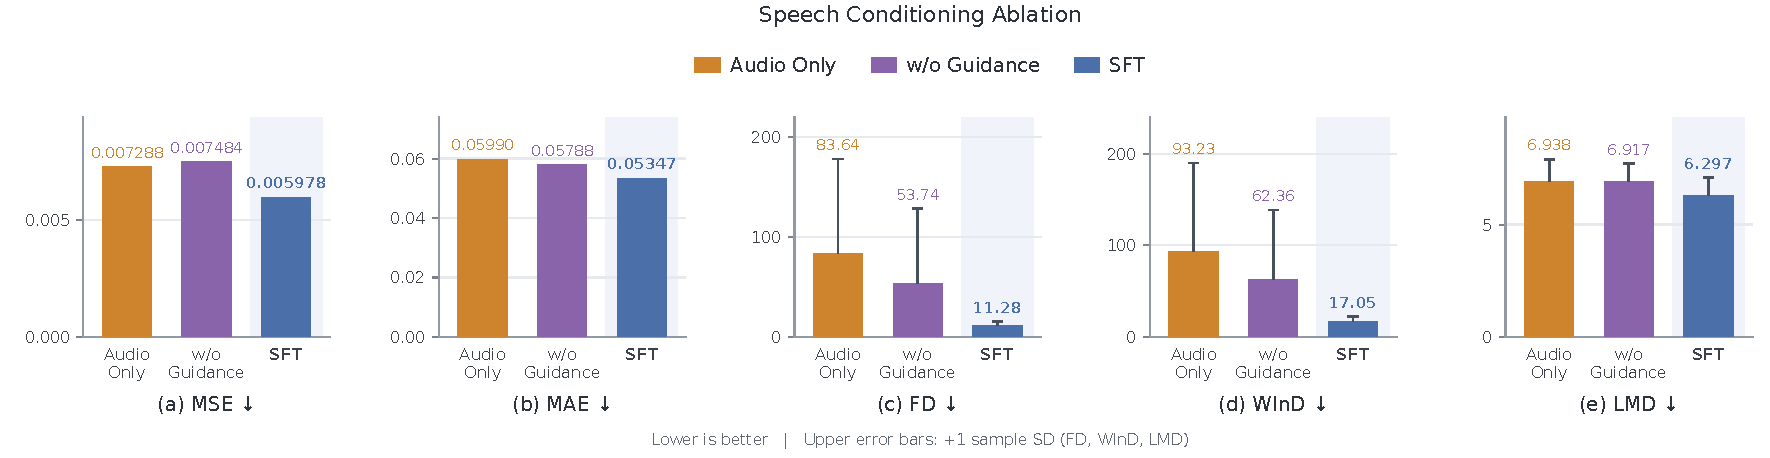
\includegraphics[width=\linewidth]{figures/ablation_conditioning_wide.pdf}
    \caption{Speech conditioning ablation. From left to right, we compare Audio Only, w/o Guidance, and the full SFT model. Results use 60 scripts from the selected test data. SFT is blue and GRPO is teal wherever shown. Lower values are better. Upper error bars show one sample standard deviation for FD, WInD, and LMD; MSE and MAE are aggregate values.}
    \label{fig:ablation_conditioning}
\end{figure}


\noindent\textbf{Ablation of Linguistic and Articulatory Conditioning.}
To examine the role of explicit linguistic inputs, we compare the full SFT generator with two variants: w/o Guidance removes articulation instructions while retaining transcripts and phonemes, and Audio Only removes all three while using the same segmented audio (Figure~\ref{fig:ablation_conditioning}).
Full conditioning gives the best overall coefficient accuracy, distributional agreement, and lip-landmark accuracy among these variants.
The two comparisons assess the contribution of articulation guidance and the joint contribution of transcript and phoneme inputs.
A plausible explanation is that linguistic cues expose speech structure, while articulation instructions connect that structure to the named facial controls, reducing the ambiguity the generator must resolve from acoustics alone.
Together, these results support conditioning structured motion generation on both linguistic content and explicit articulatory relations.

\begin{figure}[!htbp]
    \centering
    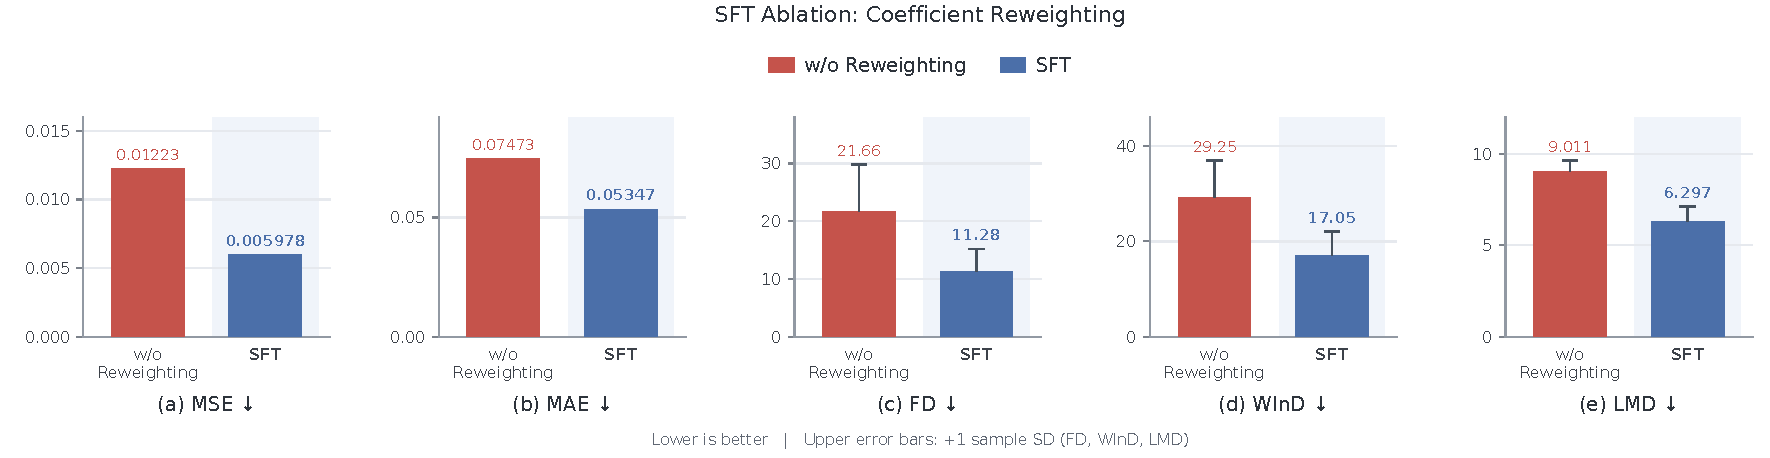
\includegraphics[width=\linewidth]{figures/ablation_reweighting_wide.pdf}
    \caption{SFT ablation of distribution-balanced supervision. The SFT model is compared with a variant using unit weights for coefficient-value tokens, with the same conditioning and post-processing. Results use 60 scripts from the selected test data. SFT is blue and GRPO is teal wherever shown. Lower values are better. Upper error bars show one sample standard deviation for FD, WInD, and LMD; MSE and MAE are aggregate values.}
    \label{fig:ablation_reweighting}
\end{figure}


\noindent\textbf{Ablation of Distribution-Balanced Supervision.}
To assess the effect of coefficient-value imbalance, we compare the weighted SFT objective with w/o Reweighting, which assigns unit weight to coefficient-value tokens while retaining the same conditioning and post-processing (Figure~\ref{fig:ablation_reweighting}).
Reweighting improves all five reported metrics, indicating benefits for both coefficient reconstruction and the resulting motion distribution and mouth shape.
This comparison evaluates the contribution of the supervised objective independently of adding linguistic inputs or GRPO refinement.
Downweighting frequent low-valued targets reduces their dominance in the loss and gives larger coefficient values greater relative emphasis during training.
The observed gains are consistent with this motivation and support distribution-balanced supervision for structured coefficient generation.

\begin{figure}[!htbp]
    \centering
    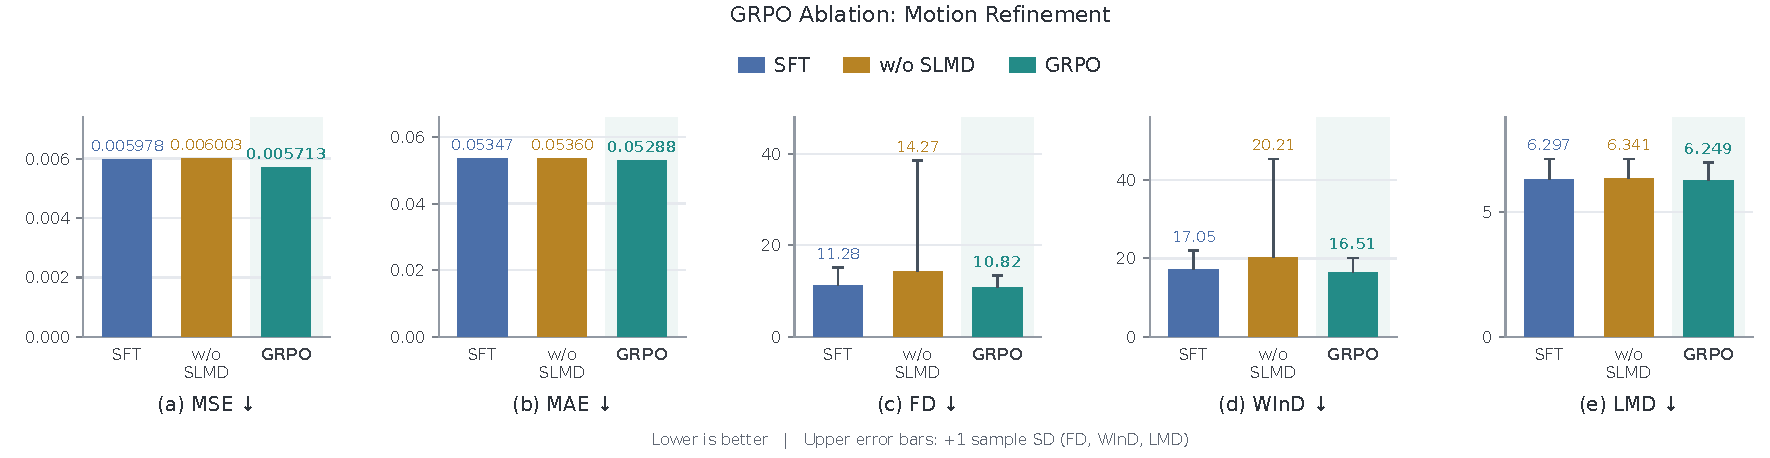
\includegraphics[width=\linewidth]{figures/ablation_motion_wide.pdf}
    \caption{GRPO ablation of motion refinement and geometric feedback. We compare SFT, GRPO refinement without SLMD, and the full refined generator under the same post-processing setting. Results use 60 scripts from the selected test data. SFT is blue and GRPO is teal wherever shown. Lower values are better. Upper error bars show one sample standard deviation for FD, WInD, and LMD; MSE and MAE are aggregate values.}
    \label{fig:ablation_motion}
\end{figure}


\noindent\textbf{Ablation of Sequence-Level Motion Refinement beyond SFT.}
To evaluate whether motion-level feedback complements token-level learning, we compare the SFT generator with Refined (GRPO) under the same post-processing setting (Figure~\ref{fig:ablation_motion}).
Refinement yields modest, consistent improvements in coefficient accuracy, distributional agreement, and lip-landmark accuracy.
This comparison assesses the additional value of sequence-level optimization after supervised adaptation.
The pattern is consistent with the reward supplying feedback on the decoded trajectory's dynamics and geometric effects, which next-token likelihood does not directly measure.
These results support using motion-aware refinement to complement the structured generation learned during SFT.

\noindent\textbf{Ablation of Explicit Geometric Mouth-Motion Feedback.}
To assess the contribution of geometric feedback within refinement, we compare the full reward with w/o SLMD, which omits the simplified 3D lip-geometry term (Figure~\ref{fig:ablation_motion}).
The full reward achieves lower mean errors across all reported metrics, whereas removing SLMD also loses the distributional gains over SFT.
This comparison examines the value of geometric supervision alongside coefficient and temporal discrepancies.
The improvement is consistent with SLMD coupling multiple controls through their combined effect on mouth deformation, a relationship that coefficient-wise errors do not represent explicitly.
The results therefore support the inclusion of geometric feedback in the refinement objective.

\section{Conclusion}
\label{sec:conclusion}

We present AudioMouth, a language-assisted framework for predicting mouth-related ARKit coefficients from speech.
Its three-stage training framework connects aligned audio-linguistic unit construction, phoneme-aware balanced supervised generation, and GRPO-based sequence-level refinement.
The refinement stage complements token-level learning with motion-level feedback, including SLMD, which evaluates coefficient-induced mouth deformation without rendering or landmark detection.
Benchmark results show competitive coefficient accuracy and strong distributional fidelity on the selected data, supporting the language-assisted formulation.

\newpage
\subsection*{AI Use Statement}

In this work, we used generative AI tools to design or provide feedback on research methodology or experiments, help develop theoretical models or conceptual frameworks, propose or refine hypotheses, implement methods, and interpret results.
We did not use generative AI tools to generate synthetic datasets, assist with translation, clean or reformat datasets, or support qualitative and thematic data analysis.
Formulating mathematical claims, providing critical ingredients for proving mathematical claims, and assisting in the writing of proofs are not applicable to this work.
Additionally, we used generative AI tools to summarize or analyze existing literature, discover research topics or identify gaps, brainstorm, and revise the wording and organization of the manuscript.
We have reviewed all AI-assisted work. For manuscript preparation, we reviewed AI-assisted drafts through iterative revision, checking that the wording and organization reflected the intended method. We also corrected the presentation of pseudocode, citation formatting, and figure captions to maintain consistency with the manuscript and figures. We take responsibility for the final content of this work, including text, claims, or artifacts produced with the aid of generative AI.

\subsection*{Ethics statement}

(This section is \textbf{recommended} and does not count toward the page limit.)

If authors feel that their paper submission raises questions regarding the Code
of Ethics, they are encouraged to include a paragraph of Ethics Statement (at
the end of the main text before references) to address potential concerns where
appropriate. Topics include, but are not limited to, studies that involve human
subjects, practices to data set releases, potentially harmful insights,
methodologies and applications, potential conflicts of interest and sponsorship,
discrimination/bias/fairness concerns, privacy and security issues, legal
compliance, and research integrity issues (e.g., IRB, documentation, research
ethics). This statement should not be more than 1 page.

\subsection*{Reproducibility Statement}

To support reproducibility, we provide detailed descriptions of the methodology, data processing, model and training configurations, reward design, baseline settings, and inference post-processing in the main text and appendix.

\newpage
\bibliography{iclr2027_conference}
\bibliographystyle{iclr2027_conference}
\newpage
\appendix
\begin{center}
{\Large AudioMouth: Language-Assisted Speech-Driven Mouth Animation with Multimodal Language Models

Supplementary Material}
\end{center}

\section{Dataset Preparation}
\label{app:dataset}

\paragraph{Source Data.}
BEAT~\cite{liu2022beat} contains 76 hours of multimodal recordings from 30 speakers across multiple languages and emotional conditions.
Its facial data comprise 52-dimensional ARKit coefficients captured at 60 Hz with an iPhone 12 Pro, synchronized with 48-kHz stereo audio.
We use its English subset.
% The result tables evaluate 60 scripts; clarify their relation to the 61 test sequences.

\paragraph{Screening.}
We render coefficient sequences with MetaHuman~\cite{metahuman} and manually inspect them together with the synchronized audio.
We discard samples with corrupted or implausible mouth motion, including occlusion-induced tracking failures, or clear audio-motion misalignment.

\paragraph{General and In-the-Wild Recordings.}
The general pipeline uses ASR to obtain transcripts and word-level timestamps, followed by SAT~\cite{frohmann2024segment} for semantic sentence segmentation. The resulting word spans define shared temporal boundaries for the audio and linguistic inputs. Where paired motion is available for training, the same boundaries select the target coefficient subsequences.

\paragraph{Benchmark Inputs.}
The source dataset provides word and phoneme annotations, which we use for the selected data in place of automatically estimated linguistic annotations. Transcript segments are matched to the word intervals in its TextGrid files; the first and last matched words determine each segment's temporal boundaries.
The same interval selects the audio, phonemes, and training coefficient subsequences.
Phonemes come from the provided annotations in all three splits, including testing, and retain CMU ARPAbet lexical stress markers (0/1/2) on vowels.
The segment transcript is constructed from the aligned words.
Target coefficient values provide training supervision and are withheld from the generator at test time.

\section{Additional Implementation Details}
\label{app:implementation}

\subsection{Coefficient Representation and JSON Format}
\label{app:json}

\paragraph{Temporal Resolution and Quantization.}
Following SAiD~\cite{park2023said}, we retain 32 mouth-related ARKit channels.
The preprocessing pipeline converts the original 60-Hz trajectories to 30 Hz by retaining every second frame within each aligned segment.
For a coefficient $v_{t,k}\in[0,1]$, the serialized integer is
\begin{equation}
q_{t,k}=\operatorname{round}(10v_{t,k})\in\{0,1,\ldots,10\}.
\end{equation}
The implementation uses Python's nearest-integer rounding, including ties to even.
Decoded integers are divided by 10 to recover coefficients on the original scale before animation post-processing.

\paragraph{Output Schema.}
Each assistant response is a JSON object with the 32 channel names below, serialized in this order. Each value is an integer array of length $T_j$, ordered chronologically at 30 Hz; every channel in a response has the same length.
The target text uses compact JSON without extra spaces. These strings are processed by the pretrained model's tokenizer.

\begin{center}
\small
\begin{tabular}{r l r l}
\hline
Index & Key & Index & Key \\
\hline
1 & \texttt{JawForward} & 17 & \texttt{MouthStretchRight} \\
2 & \texttt{JawRight} & 18 & \texttt{MouthRollLower} \\
3 & \texttt{JawLeft} & 19 & \texttt{MouthRollUpper} \\
4 & \texttt{JawOpen} & 20 & \texttt{MouthShrugLower} \\
5 & \texttt{MouthClose} & 21 & \texttt{MouthShrugUpper} \\
6 & \texttt{MouthFunnel} & 22 & \texttt{MouthPressLeft} \\
7 & \texttt{MouthPucker} & 23 & \texttt{MouthPressRight} \\
8 & \texttt{MouthRight} & 24 & \texttt{MouthLowerDownLeft} \\
9 & \texttt{MouthLeft} & 25 & \texttt{MouthLowerDownRight} \\
10 & \texttt{MouthSmileLeft} & 26 & \texttt{MouthUpperUpLeft} \\
11 & \texttt{MouthSmileRight} & 27 & \texttt{MouthUpperUpRight} \\
12 & \texttt{MouthFrownLeft} & 28 & \texttt{CheekPuff} \\
13 & \texttt{MouthFrownRight} & 29 & \texttt{CheekSquintLeft} \\
14 & \texttt{MouthDimpleLeft} & 30 & \texttt{CheekSquintRight} \\
15 & \texttt{MouthDimpleRight} & 31 & \texttt{NoseSneerLeft} \\
16 & \texttt{MouthStretchLeft} & 32 & \texttt{NoseSneerRight} \\
\hline
\end{tabular}
\end{center}

For illustration, a three-frame channel entry can be written as \texttt{"JawOpen":[2,4,3]}, corresponding to coefficients $(0.2,0.4,0.3)$. A complete response contains all 32 entries with the same array length.

\paragraph{Model Input and Training Record.}
Each JSONL training record contains a system message specifying the schema and articulation guidance, a user message with the audio placeholder, transcript, phoneme sequence, and requested frame count, and an assistant message containing the coefficient JSON as a string.
The audio file is supplied through the record's audio field.
The requested frame count defines the output duration, while the assistant coefficient sequence is the supervised target.
The articulation guidance connects phoneme groups to named controls, for example bilabial consonants to lip closure and open vowels to jaw opening.

\paragraph{Coefficient-Value Weights.}
The SFT loss uses a fixed lookup table for integers in trajectory arrays:
\begin{equation}
\omega(q)=
\begin{cases}
0.60,&q=0,\\
0.70,&q=1,\\
0.85,&q=2,\\
1.00,&q\in\{3,\ldots,10\}.
\end{cases}
\end{equation}
These are manually specified weights that reduce the contribution of frequent low-valued coefficients. JSON keys and structural punctuation retain unit weight; the reweighting applies only to array-value text.

\subsection{Model Adaptation and Training Configuration}
\label{app:training}

We initialize the generator from Qwen3-Omni-30B-A3B-Instruct~\cite{xu2025qwen3omni} and train with LoRA~\cite{hu2021lora} using four NVIDIA A100 GPUs and BF16 precision.
The audio encoder and multimodal alignment modules remain frozen in both stages.
SFT adapts the decoder's linear layers. GRPO starts from the merged SFT generator and trains new LoRA adapters on the attention query/key/value and output projections.
The two stages use the following settings; batch sizes are global across the training run, rather than per GPU.

\begin{center}
\small
\begin{tabular}{lcc}
\hline
Setting & SFT & GRPO \\
\hline
Epochs & 4 & 4 \\
LoRA rank / $\alpha$ & 32 / 32 & 8 / 16 \\
Micro-batch size & 1 & 1 \\
Global batch size & 8 & 24 \\
Learning rate & $10^{-4}$ & $10^{-6}$ \\
Minimum learning rate & $10^{-5}$ & $10^{-7}$ \\
Warmup fraction & 0.03 & 0.05 \\
Tensor parallel size & 2 & 2 \\
Context parallel size & 2 & 1 \\
Pipeline parallel size & 1 & 1 \\
\hline
\end{tabular}
\end{center}

SFT enables sequence packing with a maximum sequence length of 15,360 tokens.
GRPO permits up to 4,096 prompt tokens and 12,400 completion tokens, uses expert parallel size 4, and clips the gradient norm at 0.5.
% Epochs in both stages follow the authors' confirmed setting; the supplied
% GRPO launcher currently contains a one-epoch setting from another configuration.

\subsection{Sequence-Level Refinement}
\label{app:refinement}

\paragraph{Sampling and Policy Updates.}
GRPO samples $G=6$ candidate sequences per training prompt, with temperature 0.4, top-$p=0.95$, and repetition penalty 1.0.
The training launcher uses one policy-update iteration per sampled group, a policy-ratio clipping parameter of 0.2, and a reference-policy KL coefficient of 0.04.
The KL coefficient controls regularization separately from the four motion-reward weights.
Validation-time sampling uses four candidates per prompt.

\paragraph{Reward Normalization.}
The coefficients and scales in Eqs.~\ref{eq:normalized_score}--\ref{eq:motion_reward} are fixed during refinement:
\begin{center}
\small
\begin{tabular}{lcc}
\hline
Discrepancy & Weight $\lambda_q$ & Scale $s_q$ \\
\hline
Coefficient MSE & 0.30 & 0.660 \\
Velocity & 0.20 & 0.0380 \\
Acceleration & 0.15 & 0.0746 \\
SLMD & 0.35 & 0.0285 \\
\hline
\end{tabular}
\end{center}
The scales are stored reference-median values in the reward implementation.
FD and WInD are not reward terms. Auxiliary diagnostic scores are logged with zero optimization weight.

\paragraph{Validity and Length Handling.}
A candidate must be a parseable JSON object with the expected channels, equally long nonempty arrays, and finite integer values in $[0,10]$.
The reward assigns $-1.5$ to unparseable outputs, $-1.0$ to schema violations, and $-0.8$ to invalid numeric values.
For otherwise valid outputs, let $e_T=|T_p-T_g|/\max(T_g,1)$, where $T_p$ and $T_g$ are the predicted and reference lengths.
Candidates with $e_T>0.20$ receive $-0.6$.
For $e_T\leq0.20$, motion discrepancies are computed on the shared prefix of length $\min(T_p,T_g)$, without interpolation, and the final reward is
\begin{equation}
r=r_{\mathrm{motion}}-0.5\min(e_T,1).
\end{equation}
Thus, shorter or longer valid sequences incur a continuous penalty in addition to their motion error.

\paragraph{Fixed Geometry Asset.}
The SLMD asset is constructed from a neutral mesh and 32 ARKit blendshape meshes with identical topology.
Each basis vector is the displacement from the neutral mesh. The supplied asset retains 606 vertices from a 1,220-vertex mesh, selected using the median of nonzero aggregate deformation magnitudes over the 32 controls.
Fixed spatial weights emphasize the lip region: four nested ellipses in the neutral mesh's frontal plane assign weights of $1.0$, $0.8$, $0.6$, and $0.45$ from the innermost region outward; remaining selected vertices receive $0.1$.
Geometry is measured in the asset's native coordinate units. The basis and weights remain fixed throughout refinement.

\subsection{Inference Post-Processing}
\label{app:postprocessing}

Generated integer trajectories are decoded by dividing by 10 and assembled in temporal order on the recording timeline.
For each coefficient channel, the post-processing pipeline applies dead-zone suppression with threshold 0.02, Gaussian smoothing with standard deviation 1.0 frame and reflected boundaries, and Savitzky--Golay filtering with window length 7 and polynomial order 3.
The Savitzky--Golay filter uses interpolated boundary handling and is applied only when at least seven frames are available.
The final coefficients are clipped to $[0,1]$.

\subsection{Baseline Configuration and Visualization}
\label{app:baselines}

Audio2Face-3D~\cite{chung2025audio2face}, LAM-A2E~\cite{lam}, and SentiAvatar~\cite{jin2026sentiavatar} use publicly released pretrained weights without additional fine-tuning on our dataset.
SAiD~\cite{park2023said} is initialized from its public checkpoint and fine-tuned on our training split.
The comparison uses the mouth-related ARKit channels and speaking intervals described in Section~\ref{sec:experiments}.
Predicted coefficients are rendered with MetaHuman~\cite{metahuman} for qualitative visualization.

\section{Additional Ablation Study}
\label{app:additional_ablation}

\begin{figure}[!htbp]
    \centering
    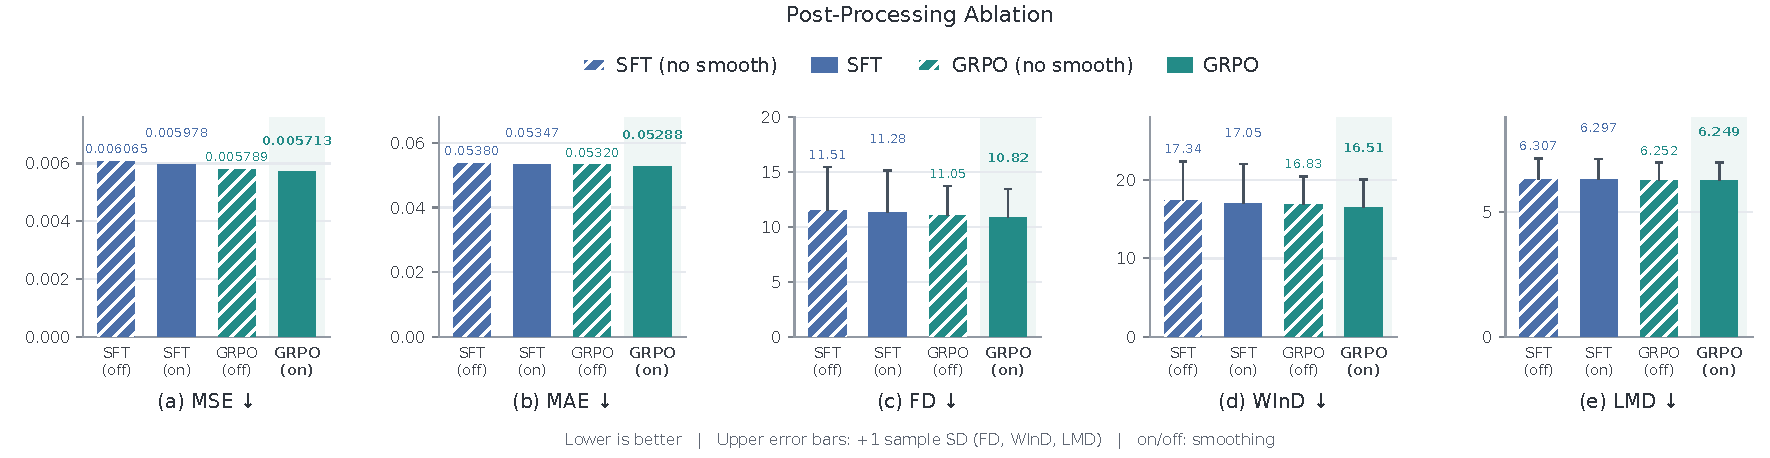
\includegraphics[width=\linewidth]{figures/ablation_smoothing_wide.pdf}
    \caption{Inference-time post-processing for SFT and Refined (GRPO). The labels on/off denote the reported settings with and without smoothing. Results use 60 scripts from the selected test data. SFT is blue and GRPO is teal; hatching identifies the no-smooth variants. Lower values are better. Upper error bars show one sample standard deviation for FD, WInD, and LMD; MSE and MAE are aggregate values.}
    \label{fig:ablation_smoothing}
\end{figure}


\noindent\textbf{Ablation of Inference-Time Post-Processing.}
To distinguish the contribution of post-processing from that of learned motion refinement, we compare SFT and Refined (GRPO) under the reported settings with and without smoothing (Figure~\ref{fig:ablation_smoothing}).
Post-processing produces small improvements across the reported metrics for both generators, while refinement remains beneficial in both settings.
The crossed comparison assesses whether the gains attributed to GRPO persist independently of smoothing.
The filtering operations can suppress local fluctuations and segment-boundary discontinuities, which is consistent with their modest complementary benefit; GRPO instead changes the generator through motion-level feedback during training.
These results support treating post-processing as a complement to motion-aware learning and show that the refinement gains persist without smoothing.

% Original table retained for reference; the figure is used in the compiled manuscript.
% \begin{table}[t]
% \centering
% {\fontsize{9}{10.5}\selectfont
% \renewcommand{\arraystretch}{1.02}
% \begin{tabular*}{\textwidth}{@{\extracolsep{\fill}} lccccc @{}}
% \hline
% \textbf{Methods}
% & \textbf{MSE $\downarrow$}
% & \textbf{MAE $\downarrow$}
% & \textbf{FD $\downarrow$}
% & \textbf{WInD $\downarrow$}
% & \textbf{LMD $\downarrow$} \\
% \hline
%
% SFT (no smooth)
% & $0.006065$
% & $0.053802$
% & $11.510 \pm 3.944$
% & $17.335 \pm 5.017$
% & $6.307 \pm 0.827$ \\
%
% SFT
% & $0.005978$
% & $0.053467$
% & $11.282 \pm 3.888$
% & $17.052 \pm 4.990$
% & $6.297 \pm 0.825$ \\
%
% Refined (no smooth)
% & $0.005789$
% & $0.053197$
% & $11.055 \pm 2.668$
% & $16.830 \pm 3.621$
% & $6.252 \pm 0.716$ \\
%
% Refined (GRPO)
% & $\mathbf{0.005713}$
% & $\mathbf{0.052878}$
% & $\mathbf{10.820 \pm 2.635}$
% & $\mathbf{16.513 \pm 3.584}$
% & $\mathbf{6.249 \pm 0.723}$ \\
% \hline
% \end{tabular*}
% }
% \caption{Training and inference-time post-processing on 60 scripts from the selected test data. ``No smooth'' denotes the reported setting without smoothing. The SFT and Refined (GRPO) rows use the standard post-processing setting. FD, WInD, and LMD are mean $\pm$ sample standard deviation across scripts. Bold marks the lowest reported value in each column.}
% \label{tab:smoothing_ablation}
% \end{table}


\section{Limitations and Future Work}
\label{app:limitations}

\paragraph{Limitations.}
The experiments on the selected data use provided word and phoneme annotations at test time. Performance with automatically recognized phonemes remains to be established. The linguistic inputs and baseline adaptation settings differ across methods, so the benchmark compares their stated configurations rather than isolating architecture alone.
The current scope is limited to 32 mouth-related ARKit coefficients and a fixed geometry basis for reward computation. Autoregressive JSON generation requires a long output sequence, and its latency has not been characterized for real-time deployment.
SLMD remains a surrogate for mouth deformation: although the completed ablation supports its contribution to refinement, it does not establish equivalence to rendered-video LMD. The reported mean differences do not establish statistical significance, and some ablated conditions exhibit substantial variation across scripts. The conditioning ablation tests transcripts and phonemes jointly and does not isolate their individual effects or the shared segmentation stage. The post-processing comparison evaluates the reported pipeline settings rather than isolating each filtering operation.
Moreover, improved facial animation techniques may also be misused for synthetic media generation, highlighting the importance of responsible deployment and appropriate safeguards.
\paragraph{Future Work.}
 
Leveraging the instruction-following ability of MLLMs, we plan to support explicit emotional control through natural language prompts, enabling richer and more expressive facial animations. We will also extend the framework to full-face coefficient generation, develop speaker-adaptive and few-shot personalization techniques, and improve robustness under in-the-wild, multilingual, and noisy conditions.



\end{document}
%弱化一些可能被攻击的表述
%删去表格的title
%实验讲述——大体总结——说明效用——解释原因——侧面证明方法
